% Definizione di un colore verde scuro personalizzato
\definecolor{darkgreen}{rgb}{0,0.5,0}  % Verde scuro RGB


% Definizione dello stile per il codice Alloy
\lstdefinelanguage{Alloy}{
    keywords={all, no, some, one, implies, and, in, not, lone, var},
    keywordstyle=\color{blue}\bfseries,
    morekeywords={assert, sig, abstract, extends, pred, run, for, but, let, set, fact, check},
    sensitive=true,
    comment=[l]{--},
    commentstyle=\color{darkgreen}\itshape,
    morestring=[b]",
    stringstyle=\color{red}
}

\lstset{
    language=Alloy,
    basicstyle=\ttfamily\small,
    numbers=none,
    numberstyle=\tiny,
    stepnumber=1,
    showstringspaces=false,
    tabsize=2,
    breaklines=true,
    breakatwhitespace=false,
    frame=none,
    keywordstyle=\color{blue}\bfseries,
    commentstyle=\color{darkgreen}\itshape,
    stringstyle=\color{red}
}


\chapter{Formal analysis using Alloy}

In our formal analysis, we have focused on modeling a dynamic system for internship management, 
incorporating both static and temporal constraints. Our model aims to represent the interplay between students, 
universities, companies, advertisements, and internships while ensuring the consistency of assignments, 
status transitions, and relationships among the entities. 

We leveraged Alloy’s temporal logic features to capture the evolution of internships and advertisements over time, 
allowing us to model preconditions, invariants, and dynamic behavior in a rigorous manner. 
The design emphasizes clarity and precision, ensuring that key system properties, such as unique assignment 
of internships and adherence to procedural rules, are verifiable.

To maintain a balance between complexity and manageability, we incorporated multiple predicates and facts 
that ensure a consistent representation of system behaviors, such as application processing, advertisement closure, 
and feedback provision. Temporal constraints, such as ensuring no return to previous states (e.g., WAITING) 
or eventual resolution of complaints, were introduced to demonstrate the system's progression over time without 
overcomplicating the analysis. This approach enabled us to comprehensively capture the problem's intricacies while 
facilitating the exploration of its temporal dynamics.


\section{Alloy Code}


\begin{lstlisting}
-------------------- DEFINITION OF ENUM --------------------

enum InternshipStatus {WAITING, ONGOING, REVIEW, FINISHED}
enum Bool {true, false}
    
    
-------------------- DEFINITION OF SIGNATURES --------------------



abstract sig User {}
    
sig Student extends User {
    skills: set Skill,
    var assignedInternship: lone Internship,
}{
	 #skills > 0
}

sig Company extends User {
	advertisement : set Advertisement,
}

sig University extends User {
    students: set Student,
}

sig Advertisement {
    requirements: set Skill,
    description: one Description,
    spots: one Int,
    var applicants: set Student,
    var assigned: one Bool,
    internship: set Internship,
}{
    spots >= 1 and spots <= 3 
}

sig Internship {
    offeredBy: one Company,
    var assignedTo: lone Student,
    var feedback: lone Feedbacks,
    var status: one InternshipStatus,
}

sig Feedbacks {}

sig Description{}

sig Skill {}

-----------------------------PREDICATES------------------------------

-- This predicate handles the application of a student to an advertisement
pred Apply[s: Student, a: Advertisement] {
    -- Precondition: all internships related to the advertisement must have a status of WAITING
    all i: a.internship |
        i.status = WAITING

    -- No changes allowed 
    a.assigned' = a.assigned
    all i: a.internship | {
        i.status' = i.status and
        i.assignedTo' = i.assignedTo
    }

    -- Postcondition: the student is added to the list of applicants
    a.applicants' = a.applicants + s
}

-- This predicate closes an advertisement and assigns internships to applicants
pred CloseAdv[a: Advertisement] {
    -- Precondition: the number of applicants must be greater than or equal to the available spots, and the advertisement is not yet assigned
    #a.applicants >= a.spots
    a.assigned = false
    all i: a.internship |
        i.status = WAITING

    -- No changes allowed 
    a.applicants' = a.applicants

    -- Postcondition: the advertisement is marked as assigned, and internships are assigned
    a.assigned' = true
    AssignInternship[a]
}

-- This predicate assigns internships to students in an advertisement
pred AssignInternship[a: Advertisement] {
    -- Precondition: the number of applicants must be greater than or equal to the available spots, and the advertisement is not yet assigned
    #a.applicants >= a.spots
    a.assigned = false
    all i: a.internship |
        i.status = WAITING

    -- Postcondition: every internship is assigned to a unique student
    all i: a.internship | {
        some s: a.applicants | {
            i.assignedTo' = s and
            assignedInternship' = ~assignedTo'
        }
    }

    -- Ensure that each internship is assigned to a different student
    all disj i1, i2: a.internship |
        i1.assignedTo' != i2.assignedTo'

    -- Update the status of all internships to ONGOING
    all i: a.internship |
        i.status' = ONGOING
}

-- This predicate closes an internship, marking it as finished
pred CloseInternship[i: Internship] {
    -- Precondition: the internship must have a status of ONGOING
    i.status = ONGOING

    -- No changes allowed to the assigned student
    i.assignedTo' = i.assignedTo

    -- Postcondition: the internship status is updated to FINISHED, and feedback is provided
    i.status' = FINISHED
    some i.feedback'
}

-- This predicate opens a complaint for an internship 
pred OpenComplaint[i: Internship] {
    -- Precondition: the internship must have a status of ONGOING
    i.status = ONGOING

    -- No changes allowed 
    i.assignedTo' = i.assignedTo
    i.assignedTo.assignedInternship' = i.assignedTo.assignedInternship

    -- Postcondition: the internship status is updated to REVIEW
    i.status' = REVIEW
}

-- This predicate resolves a complaint for an internship
pred ResolveComplaint[i: Internship] {
    -- Precondition: the internship must have a status of REVIEW
    i.status = REVIEW

    -- No changes allowed 
    i.assignedTo' = i.assignedTo
    i.assignedTo.assignedInternship' = i.assignedTo.assignedInternship

    -- Postcondition: the internship status is updated to either ONGOING or FINISHED
    i.status' = ONGOING or i.status' = FINISHED
}


------------------------INITIAL DYNAMIC CONDITIONS------------------------

-- Ensures that initially, no student is assigned to any internship
fact InitialConditionStudent {
    all s: Student |
        no s.assignedInternship
}

-- Ensures that initially, no advertisement has any applicants, and none are assigned
fact InitialConditionAdv {
    all a: Advertisement | {
        #a.applicants = 0 and
        a.assigned = false
    }
}

-- Ensures that initially, internships have no assigned students, no feedback, and are in a WAITING state
fact InitialConditionInternship {
    all i: Internship |{
        no i.assignedTo and
        no i.feedback and
        i.status = WAITING
    }
}


-----------------------------STATIC FACTS------------------------------

-- Ensures that the number of spots in an advertisement equals the number of internships associated with it
fact SpotForInternship {
    all a: Advertisement |
        a.spots = #a.internship
}

-- Ensures that each internship is associated with exactly one advertisement
fact UniqueAdvertisementForEachInternship {
    all i: Internship | 
        one a: Advertisement | i in a.internship
}

-- Ensures that each student belongs to one and only one university
fact UniqueUniversityPerStudent {
    all s: Student | {
        one u: University | s in u.students and
        all disj u1, u2: University | {
            s in u1.students => s not in u2.students
        }
    }
}

-- Ensures that no university is empty; every university must have at least one student
fact NoEmptyUniversity {
    all u: University | some u.students
}

-- Ensures that each advertisement belongs to exactly one company
fact UniqueCompanyPerAdvertisement {
    all a: Advertisement | {
        one c: Company | a in c.advertisement and
        all disj c1, c2: Company | {
            a in c1.advertisement => a not in c2.advertisement
        }
    }
}

-- Ensures that no company is empty; every company must have at least one advertisement
fact NoEmptyCompany {
    all c: Company | some c.advertisement
}

-- Ensures that internships are offered by the company that published their associated advertisement
fact ConsistentCompanyAdvertisementInternship {
    all c: Company | all a: c.advertisement | {
        all i: a.internship | i.offeredBy = c
    }
}

-- Ensures that all advertisements have unique descriptions
fact UniqueDescriptions {
    all disj a1, a2: Advertisement | a1.description != a2.description
}

-- Ensures that the number of the Feedbacks is equal to the number of Internship
fact NumOfInternshipMatchNumOfFeedback {
	#Feedbacks = #Internship
}


--------------------------ALWAYS TRUE FACTS------------------------------

-- Ensures that once an internship is marked as FINISHED, it will always not change
fact InternshipStayFinished {
    all i: Internship | 
        always (i.status = FINISHED => some i.feedback and 
            always (i.status = FINISHED and i.feedback' = i.feedback ))
}

-- Ensures that once an advertisement is assigned, it will always remain assigned and its list of applicants will not change
fact AdvertisementStayClose {
    all a: Advertisement |
        always (a.assigned = true => always (a.assigned = true and a.applicants' = a.applicants))
}

-- Ensures that internships in certain statuses (ONGOING, REVIEW, FINISHED) always have an assigned student, and those in WAITING have no assigned student
fact AssignedStatusConsistency {
    all i: Internship |
        always (i.status in (ONGOING + REVIEW + FINISHED) => some i.assignedTo and i.assignedTo' = i.assignedTo) and
        always (i.status = WAITING => no i.assignedTo)
}

-- Ensures that internships in ONGOING or REVIEW statuses always have their assigned student linked to that internship
fact InternshipAssignedStudentConsistency {
    all i: Internship |
        always (i.status in (ONGOING + REVIEW) => i.assignedTo.assignedInternship = i)
}

-- Ensures that a student cannot have an assigned internship before it starts or after it is finished
fact ValidStudentAssignment {
    all s: Student | 
        always (some s.assignedInternship => s.assignedInternship.status in (ONGOING + REVIEW))
}

-- Ensures consistent historical state transitions for internships
fact CheckStateHistory {
    all i: Internship | {
        always (i.status = ONGOING => once i.status = WAITING)
        always (i.status = REVIEW => once i.status = ONGOING)
        always (i.status = FINISHED => once i.status = ONGOING)
    }
}

-- Ensures that if an advertisement is not assigned, all its internships must be in the WAITING state
fact AdvOpen {
    all a: Advertisement |
        always (a.assigned = false => (all i: a.internship | i.status = WAITING))
}

-- Ensures that once an internship leaves the WAITING state, it cannot return to it
fact NoReturnToWaiting {
    all i: Internship | always (once (i.status != WAITING) => always (i.status != WAITING))
}

-- Ensures that any student assigned to an internship must have applied to its advertisement
fact AssignedStudentApplied {
    always (all i: Internship | {
        some i.assignedTo => some a: Advertisement | {
            i in a.internship and i.assignedTo in a.applicants
        }
    })
}

-- Ensures that feedback can only be given after an internship is finished
fact NoFeedbackBeforeFinished {
    always (all i: Internship | {
        i.status != FINISHED => no i.feedback
    })
}

-- Ensures that feedback is unique for each internship
fact UniqueFeedbackPerInternship {
    always (all disj i1, i2: Internship | 
        i1.status = FINISHED and i2.status = FINISHED => i1.feedback != i2.feedback)
}


----------------------------DYNAMIC FACTS-------------------------------

-- Ensures that if an advertisement is not assigned, eventually a student will apply to it
fact EventuallyApply {
    all a: Advertisement | {
        a.assigned = false => eventually (some s: Student | 
            no s.assignedInternship and s not in a.applicants and Apply[s, a])
    }
}

-- Ensures that if an advertisement is not assigned, it will eventually be closed
fact EventuallyCloseAdv {
    all a: Advertisement |
        a.assigned = false => eventually (CloseAdv[a])
}

-- Ensures that all internships will eventually be closed
fact EventuallyCloseInternship {
    all i: Internship |
        eventually (CloseInternship[i])
}

-- Ensures that eventually, at least one internship will have a complaint opened
fact EventuallyOpenComplaint {
    some i: Internship | 
        eventually OpenComplaint[i]
}

-- Ensures that internships in the REVIEW state will have their complaints resolved
fact AlwaysResolveComplaint {
    all i: Internship | {
        always (i.status = REVIEW => ResolveComplaint[i])
    }
}


-----------------------------ASSERTIONS----------------------------------

-- Ensures that an internship can only be assigned to a student if the student has applied to the associated advertisement
assert InternshipAssignmentRequiresApplication {
    all i: Internship | 
    some i.assignedTo => some a: Advertisement | 
        i in a.internship and i.assignedTo in a.applicants
}

-- Ensures that internships follow the exact state sequence: WAITING -> ONGOING -> REVIEW (optional) -> FINISHED, without skipping or repeating states
assert ExactStateSequence {
    all i: Internship | {
        always (i.status = WAITING => not once (i.status in (ONGOING + REVIEW + FINISHED)))
        always (i.status = ONGOING => once (i.status = WAITING) and not once (i.status = FINISHED))
        always (i.status = REVIEW => once (i.status in (ONGOING + WAITING) and not once (i.status = FINISHED)))
        always (i.status = FINISHED => once (i.status = REVIEW or i.status = ONGOING))
    }
}

-- Ensures that if an internship enters the REVIEW state, it will transition to the FINISHED state
assert ReviewEventuallyLeadsToFinished {
    all i: Internship | {
        once (i.status = REVIEW) => always (i.status = FINISHED)
    }
}

-- Ensures that an advertisement can only be closed if all its internships are assigned
assert NoClosedAdvertisementWithoutAssignedInternships {
    all a: Advertisement | 
    a.assigned = true => all i: a.internship | some i.assignedTo
}

-- Ensures that each student is assigned to only one internship at a time
assert UniqueAssignmentPerStudent {
    always (all disj i1, i2: Internship | 
        (i1.status != WAITING and i2.status != WAITING) => i1.assignedTo != i2.assignedTo)
}


-------------------------------RUN-----------------------------------

check InternshipAssignmentRequiresApplication for 5
check ExactStateSequence for 5
check ReviewEventuallyLeadsToFinished for 5
check NoClosedAdvertisementWithoutAssignedInternships for 5
check UniqueAssignmentPerStudent for 5

pred show {
    #Advertisement = 2
    #internship = 5
    #University = 2
    #Company = 2
    #Student = 6
    #Skill = 2
    eventually (one i: Internship | i.status = REVIEW)
}

run show for 10


\end{lstlisting}


\section{Assertion Results}

\begin{figure}[H]
    \centering
    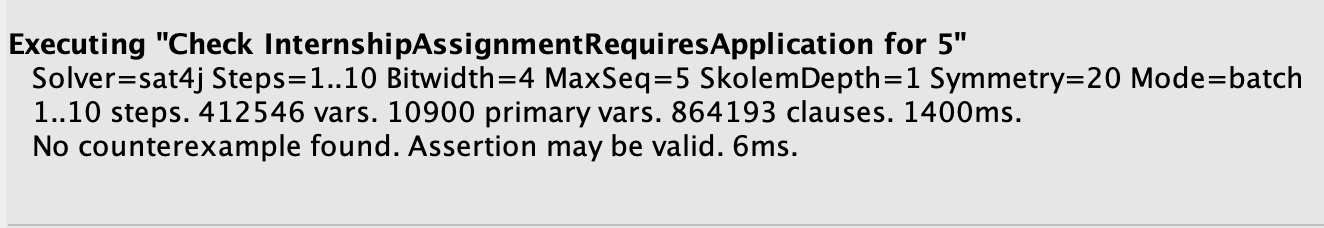
\includegraphics[width=350px]{../../assets/alloy-assertion/I_assertion.png}
    \caption{An Internship can only be assigned to a student if the student has applied to the associated advertisement}
\end{figure}

\begin{figure}[H]
    \centering
    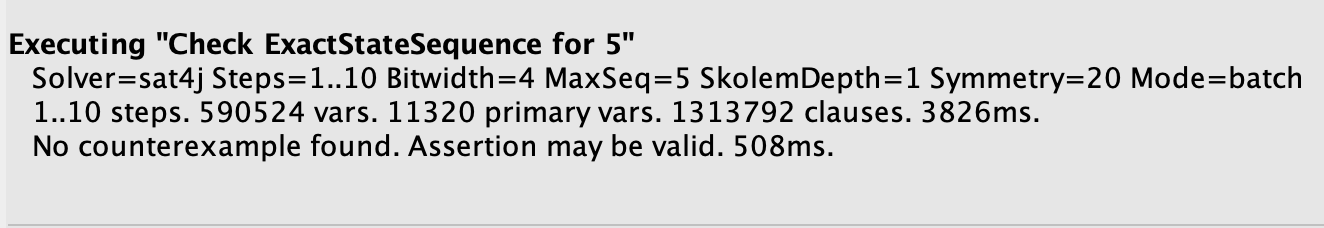
\includegraphics[width=350px]{../../assets/alloy-assertion/II_assertion.png}
    \caption{Internships follow the exact temporal sequence}
\end{figure}

\begin{figure}[H]
    \centering
    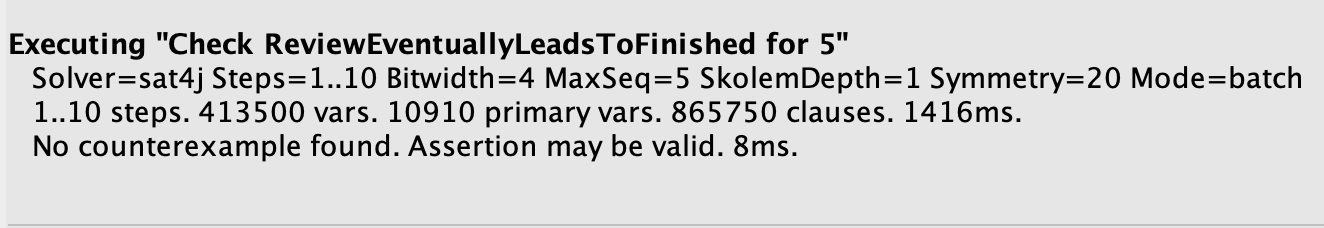
\includegraphics[width=350px]{../../assets/alloy-assertion/III_assertion.png}
    \caption{if an internship enters the REVIEW state, it will transition to the FINISHED state}
\end{figure}


\begin{figure}[H]
    \centering
    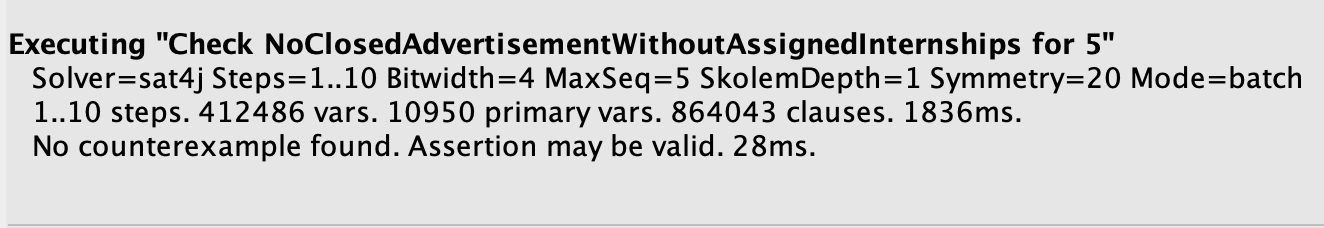
\includegraphics[width=350px]{../../assets/alloy-assertion/IV_assertion.png}
    \caption{An advertisement can only be closed if all its internships are assigned}
\end{figure}

\begin{figure}[H]
    \centering
    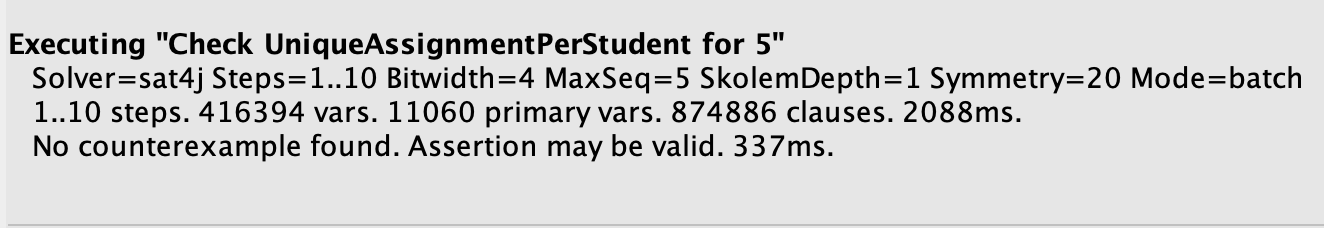
\includegraphics[width=350px]{../../assets/alloy-assertion/V_assertion.png}
    \caption{Each student is assigned to only one internship at a time}
\end{figure}



\section{World Generated}
 
 
\begin{figure}[H]
    \centering
    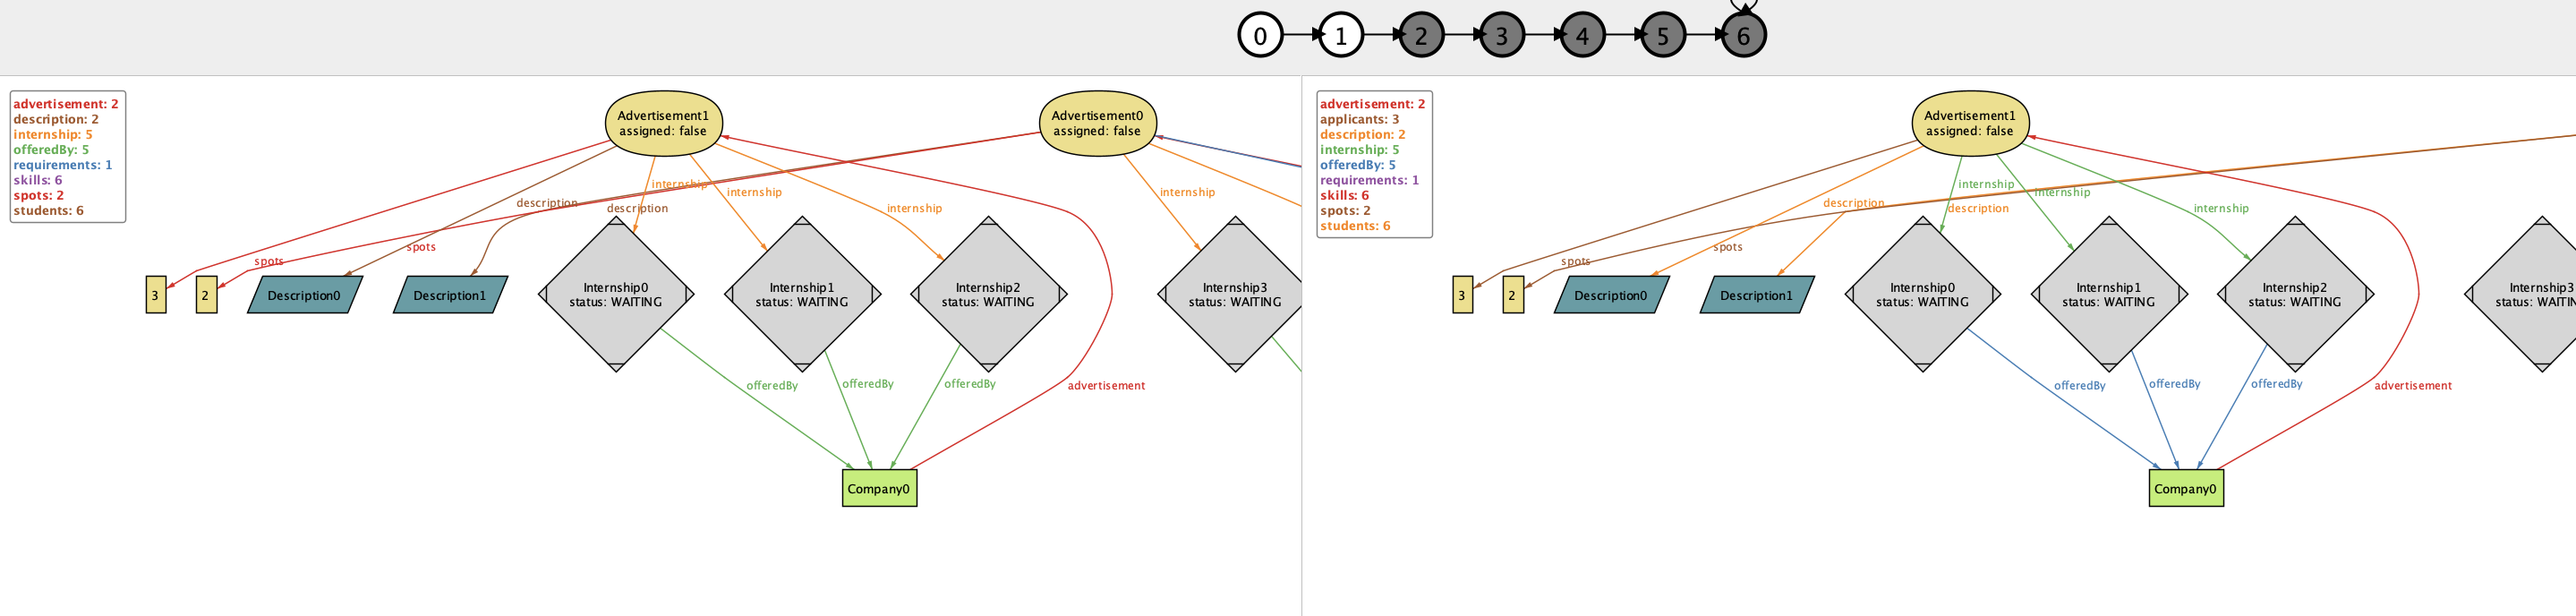
\includegraphics[width=450px]{../../assets/alloy-world/world_steps.png}
    \caption{show the total temporal steps}
\end{figure}

\begin{figure}[H]
    \centering
    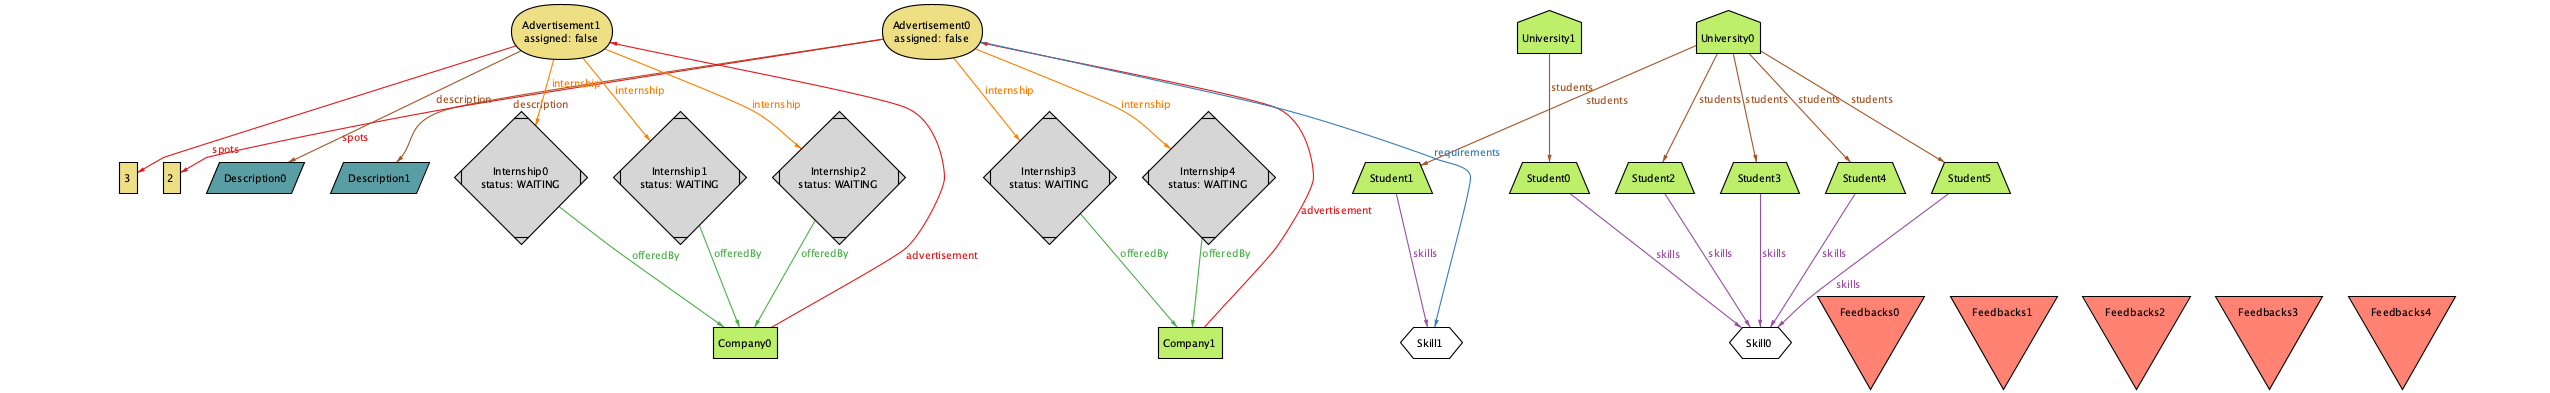
\includegraphics[width=450px]{../../assets/alloy-world/I_step.png}
    \caption{I - Temporal step}
\end{figure}

\begin{figure}[H]
    \centering
    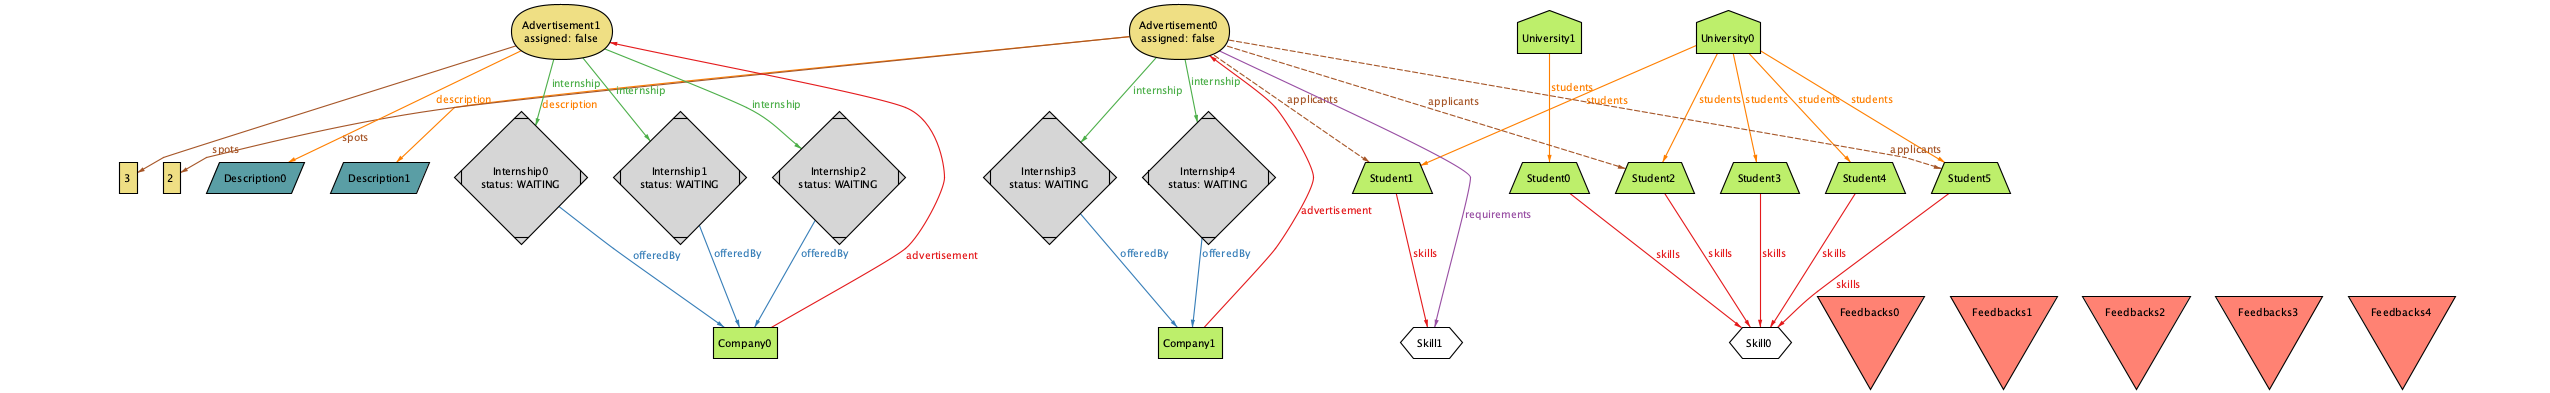
\includegraphics[width=450px]{../../assets/alloy-world/II_step.png}
     \caption{II - Temporal step}
\end{figure}


\begin{figure}[H]
    \centering
    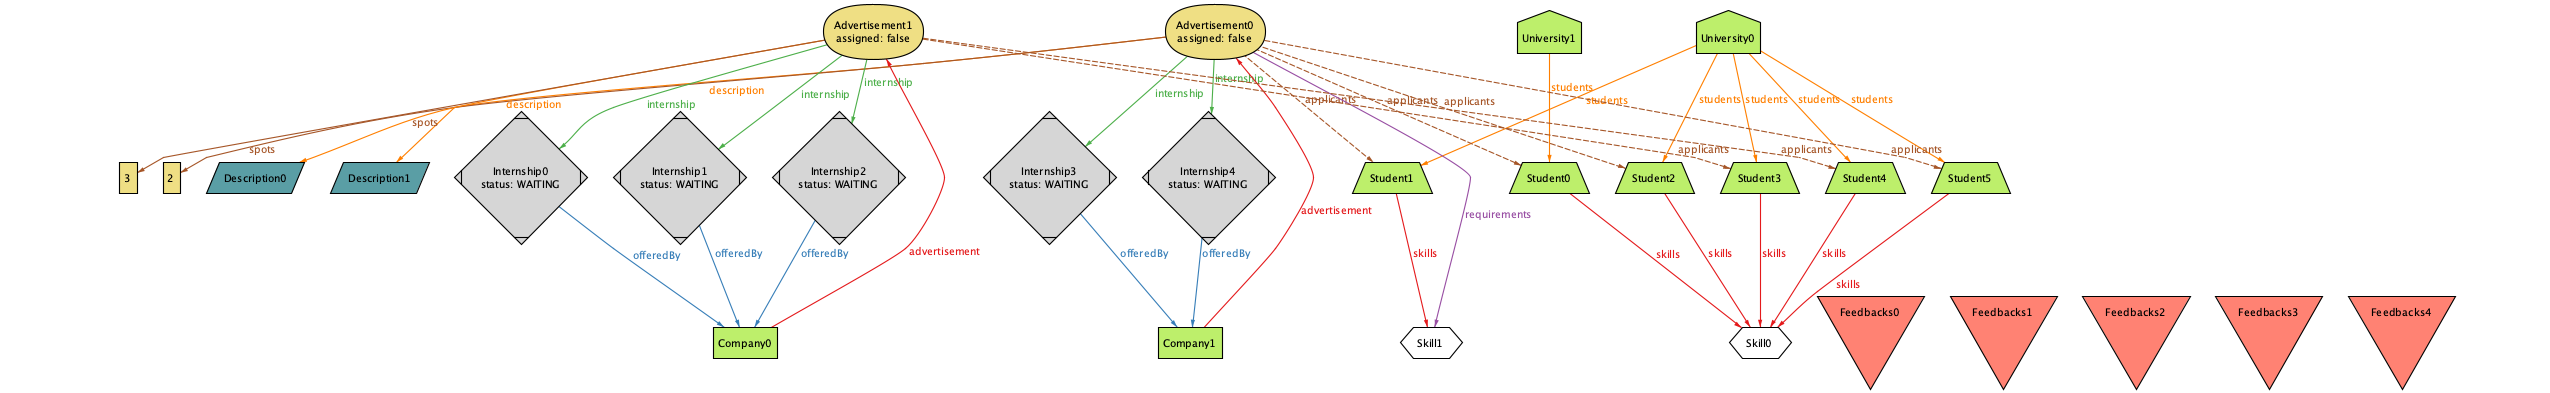
\includegraphics[width=450px]{../../assets/alloy-world/III_step.png}
    \caption{III - Temporal step}
\end{figure}

\begin{figure}[H]
    \centering
    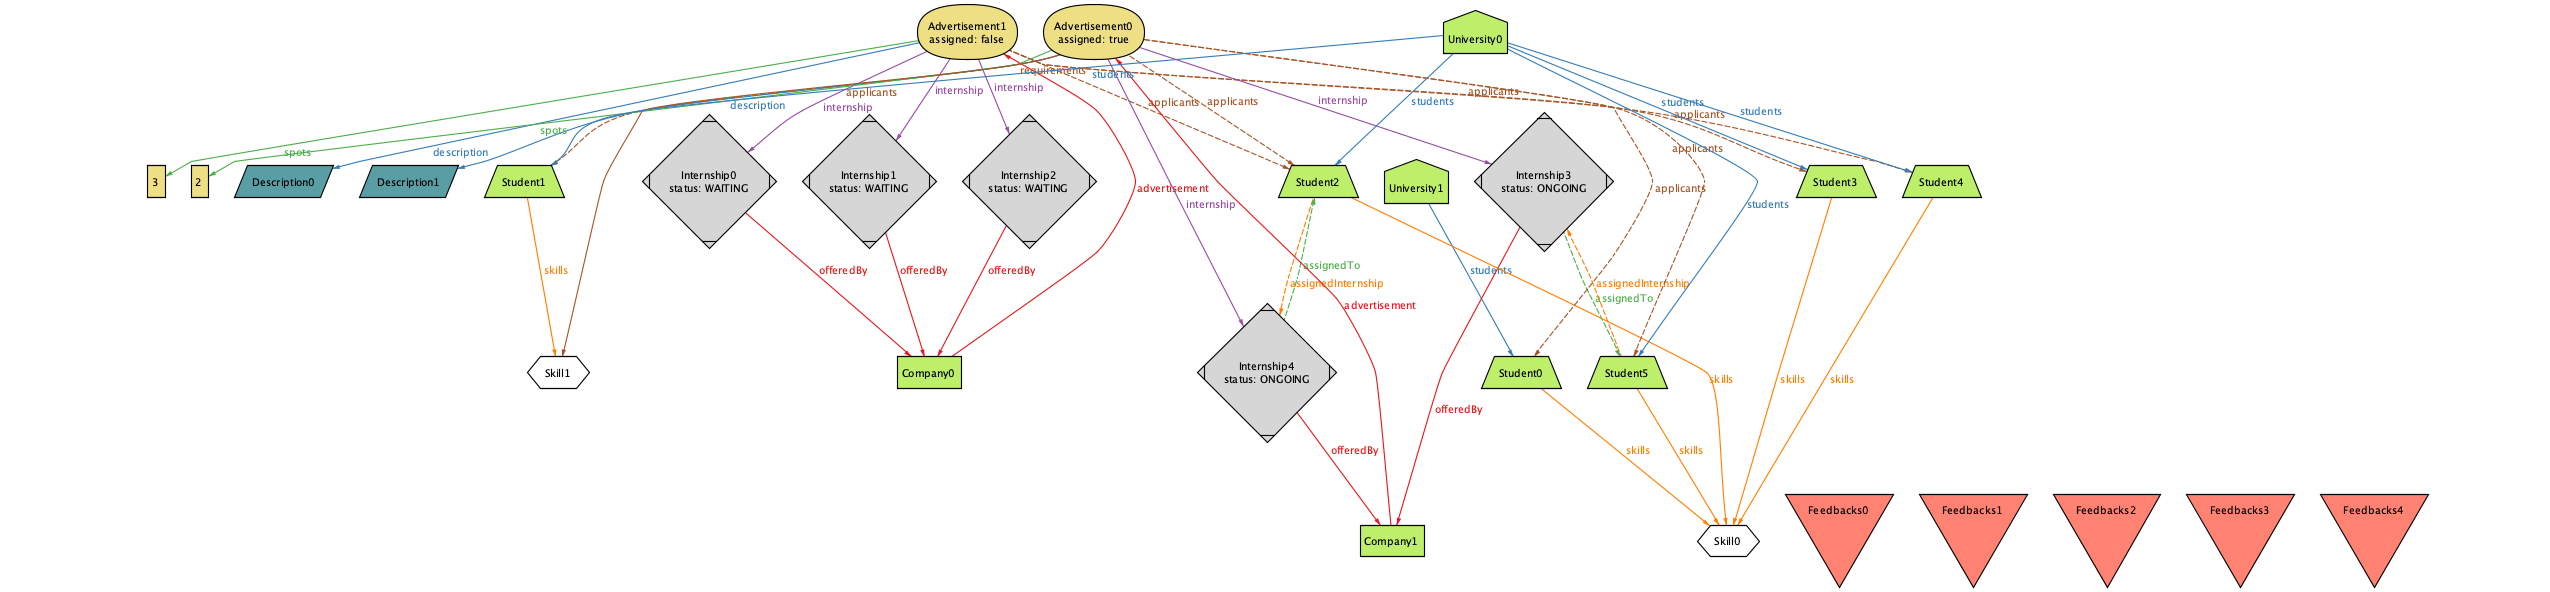
\includegraphics[width=450px]{../../assets/alloy-world/IV_step.png}
    \caption{IV - Temporal step}
\end{figure}

\begin{figure}[H]
     \centering
     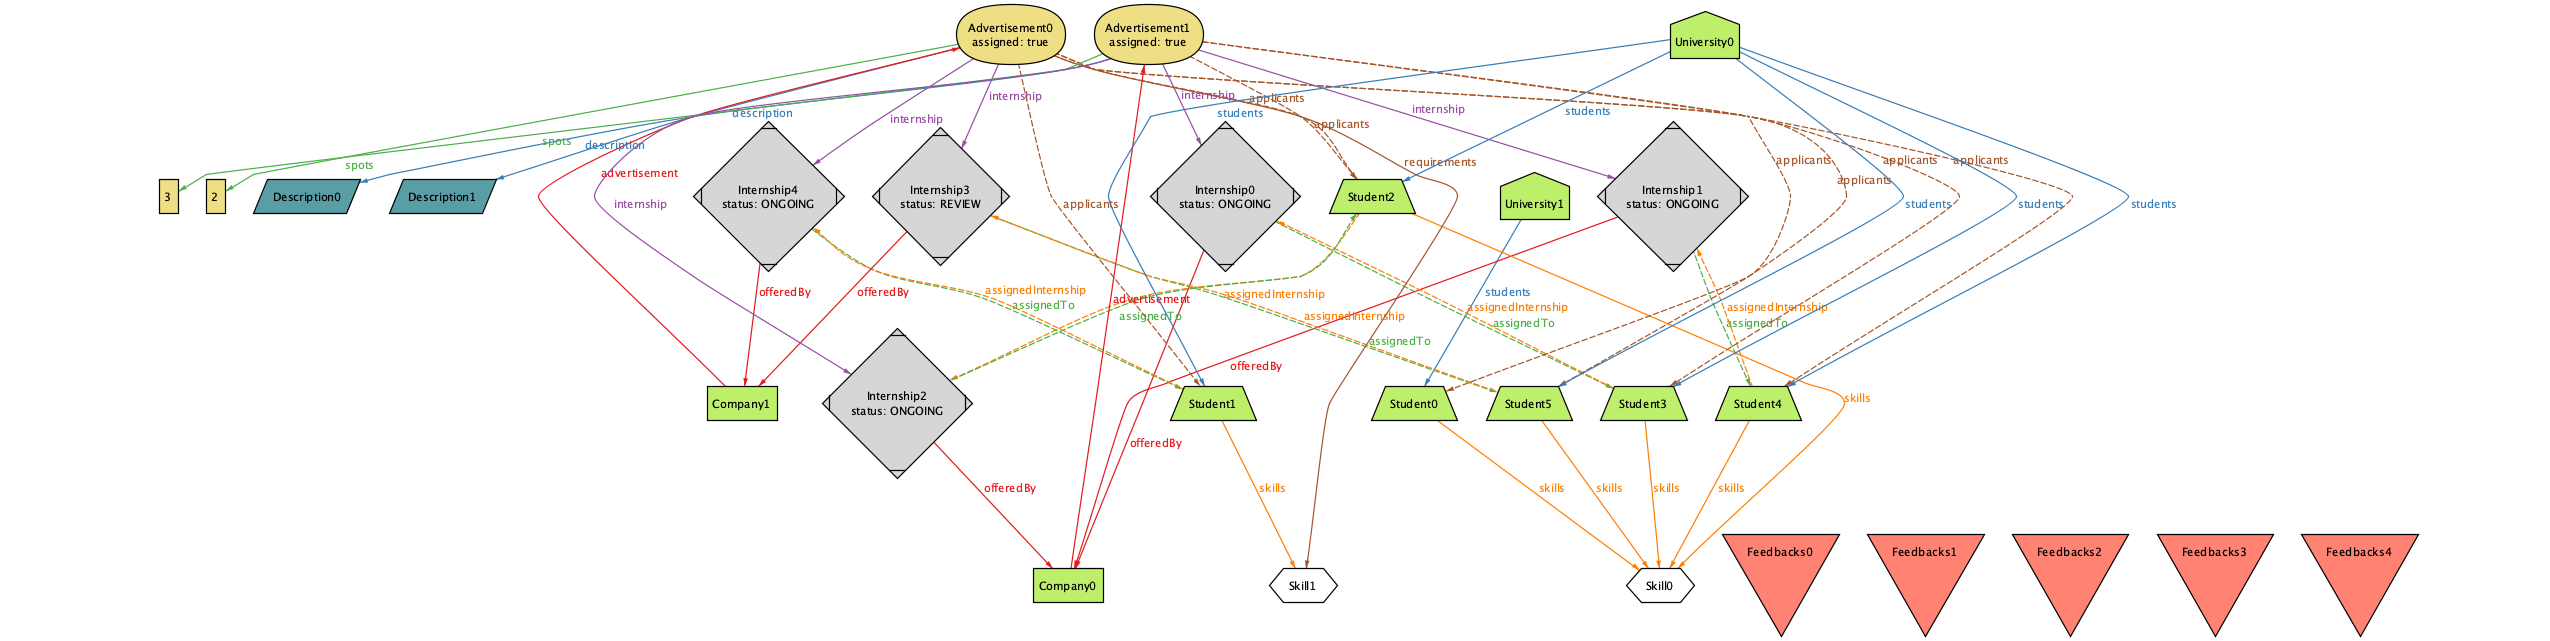
\includegraphics[width=450px]{../../assets/alloy-world/V_step.png}
     \caption{V - Temporal step}
\end{figure}

\begin{figure}[H]
     \centering
     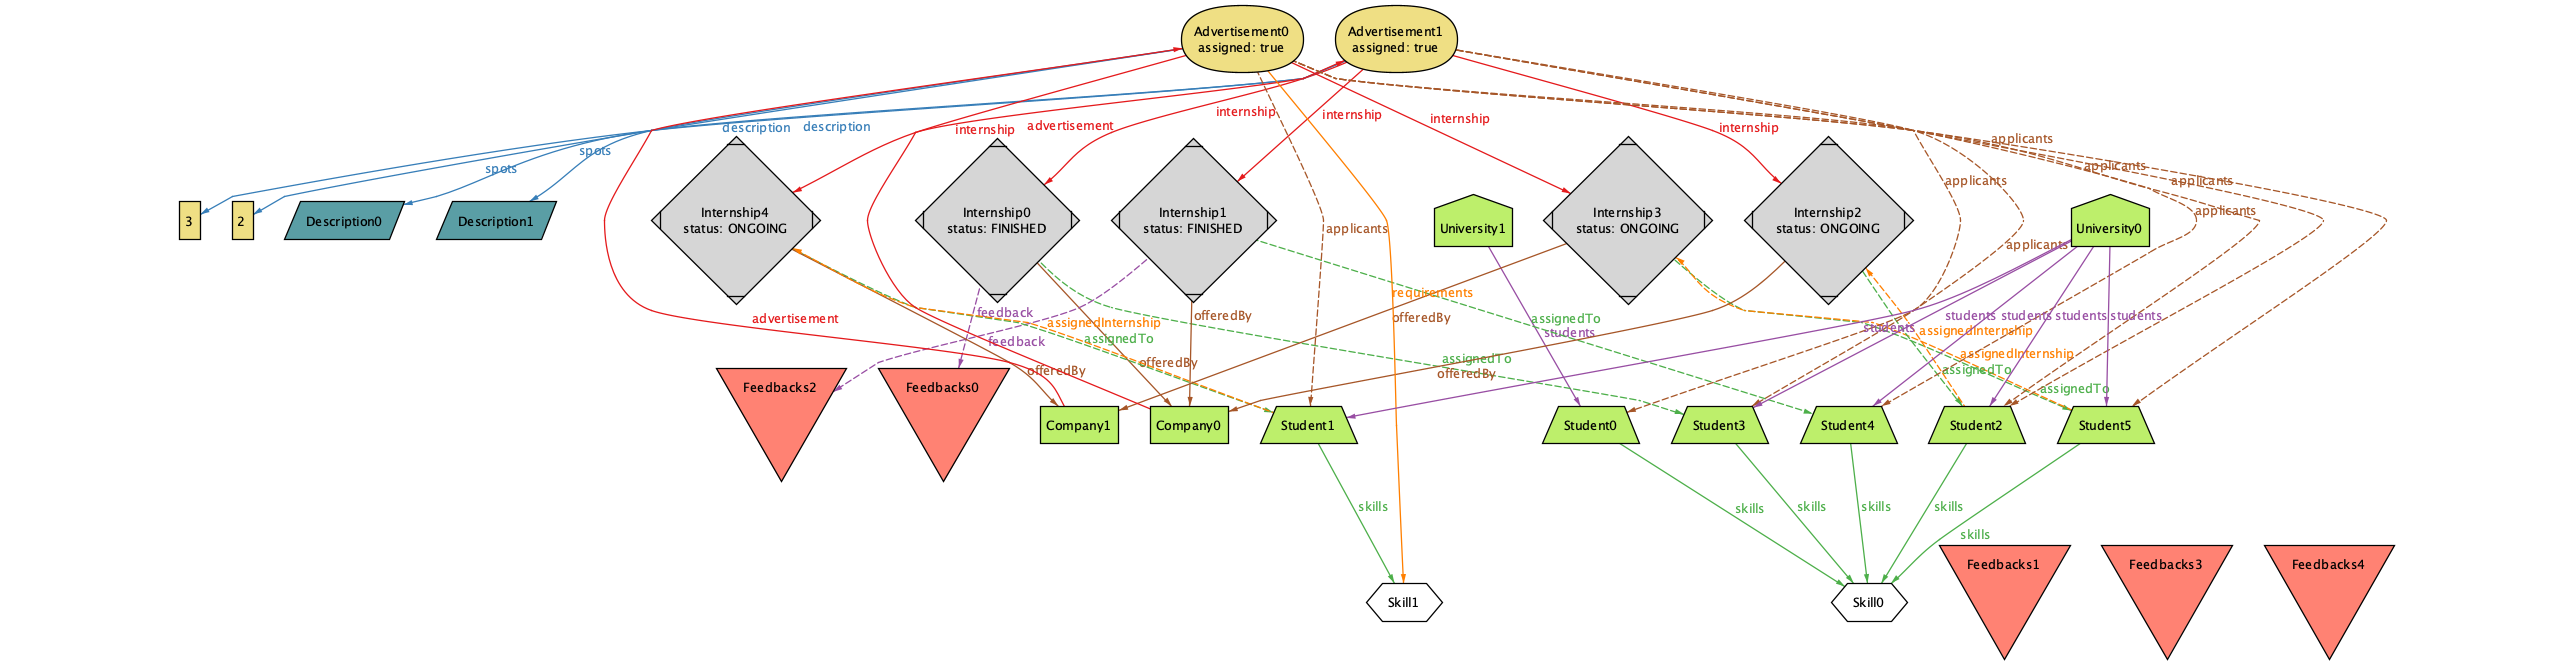
\includegraphics[width=450px]{../../assets/alloy-world/VI_step.png}
     \caption{VI - Temporal step}
\end{figure}

\begin{figure}[H]
     \centering
     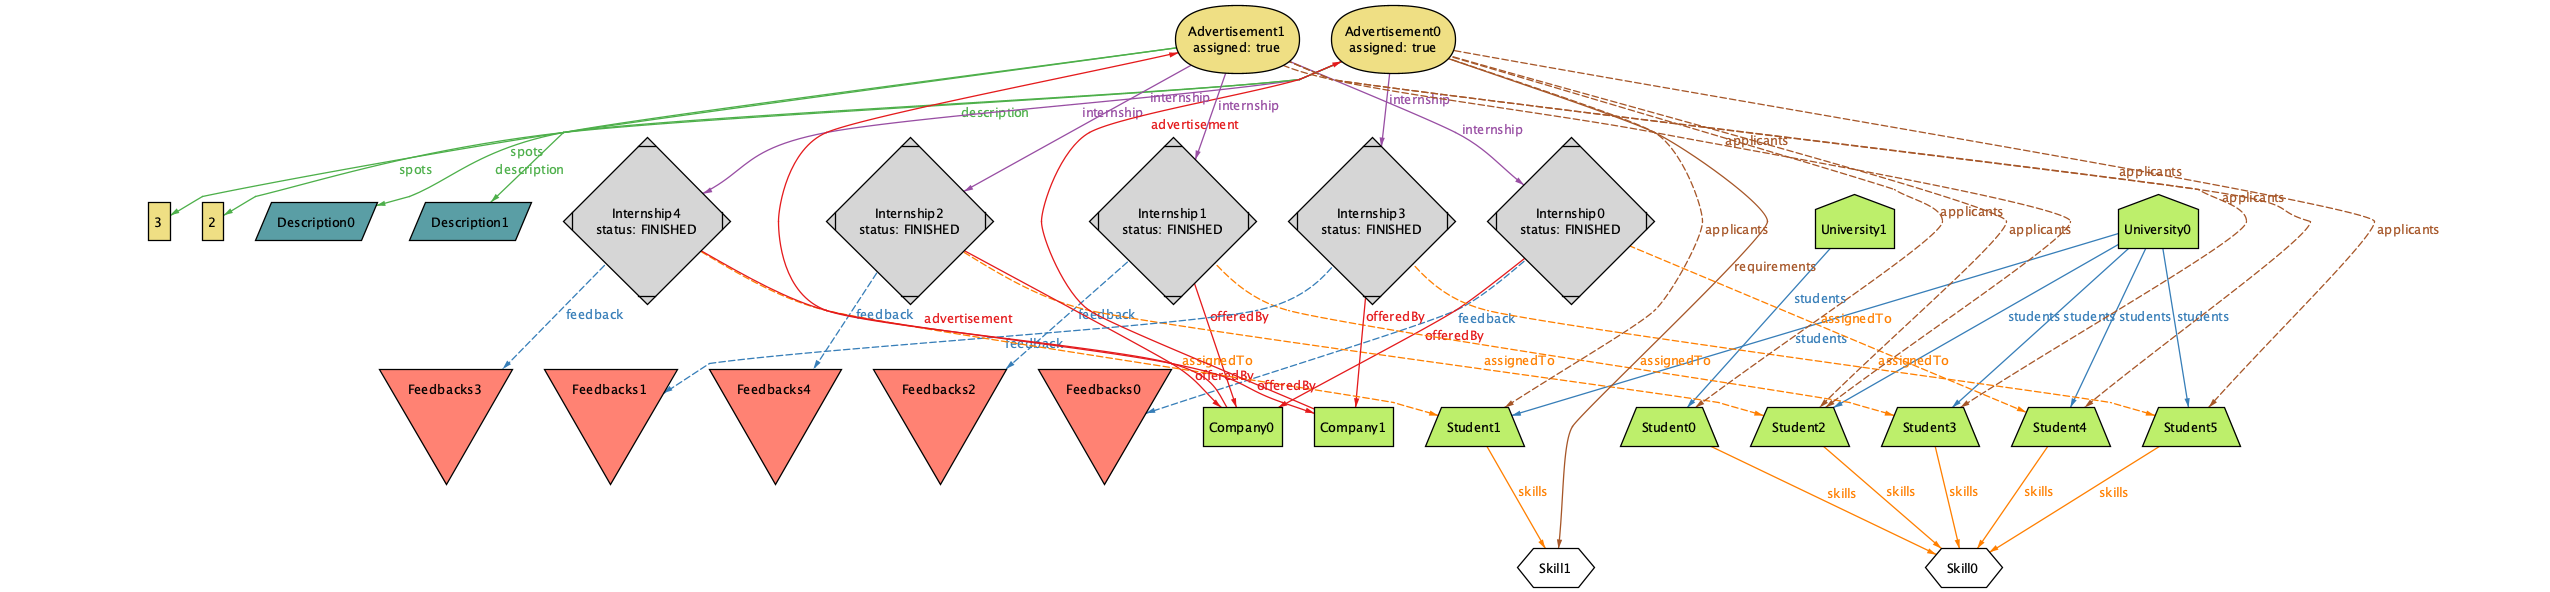
\includegraphics[width=450px]{../../assets/alloy-world/VII_step.png}
     \caption{VII - Temporal step}
\end{figure}


